\section{Aufbau}
\label{sec:Aufbau}

\begin{figure}
 \centering
 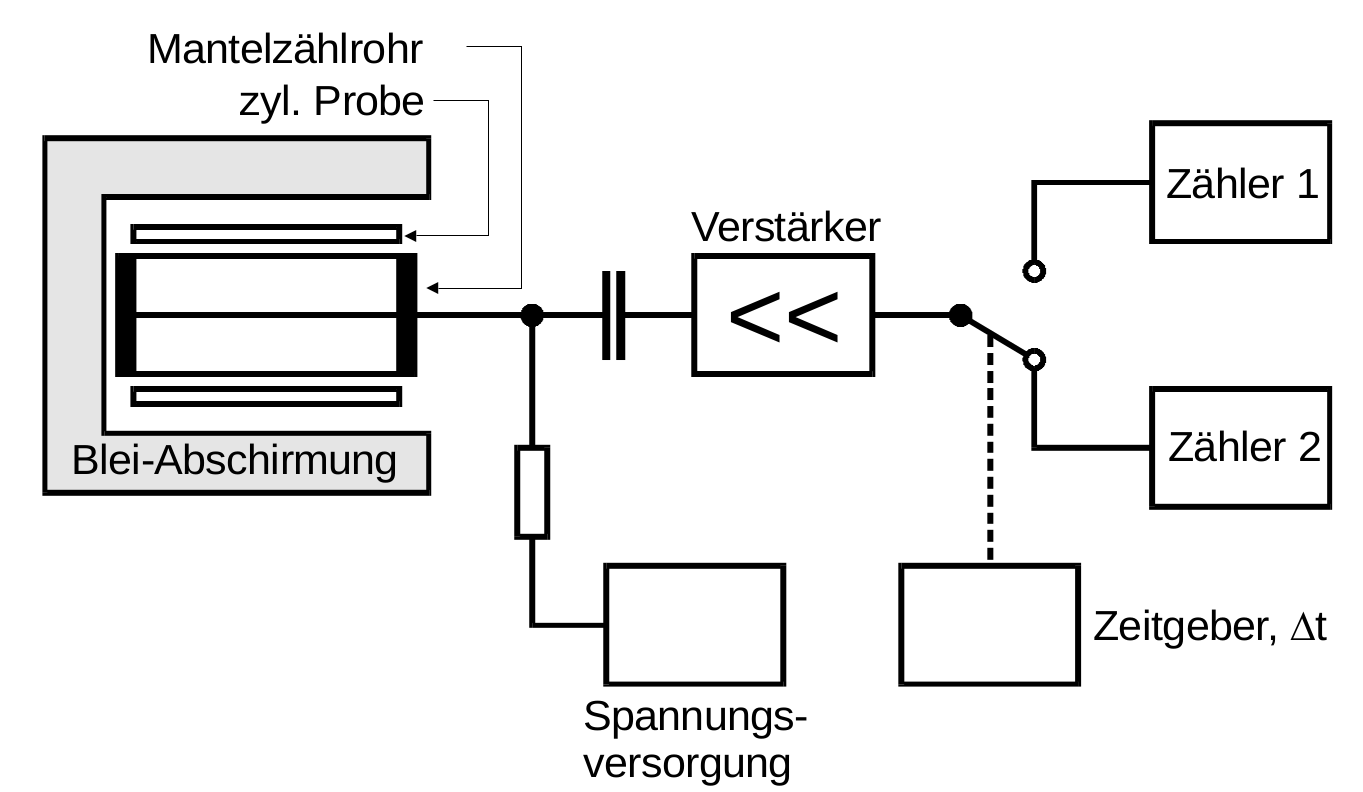
\includegraphics[width=\linewidth-70pt,height=\textheight-70pt,keepaspectratio]{content/aufbau.png}
  \caption{Eine schematische Darstellung des Messaufbaus \cite{V702}}
 \label{fig:aufbau}
\end{figure}

\begin{figure}
 \centering
 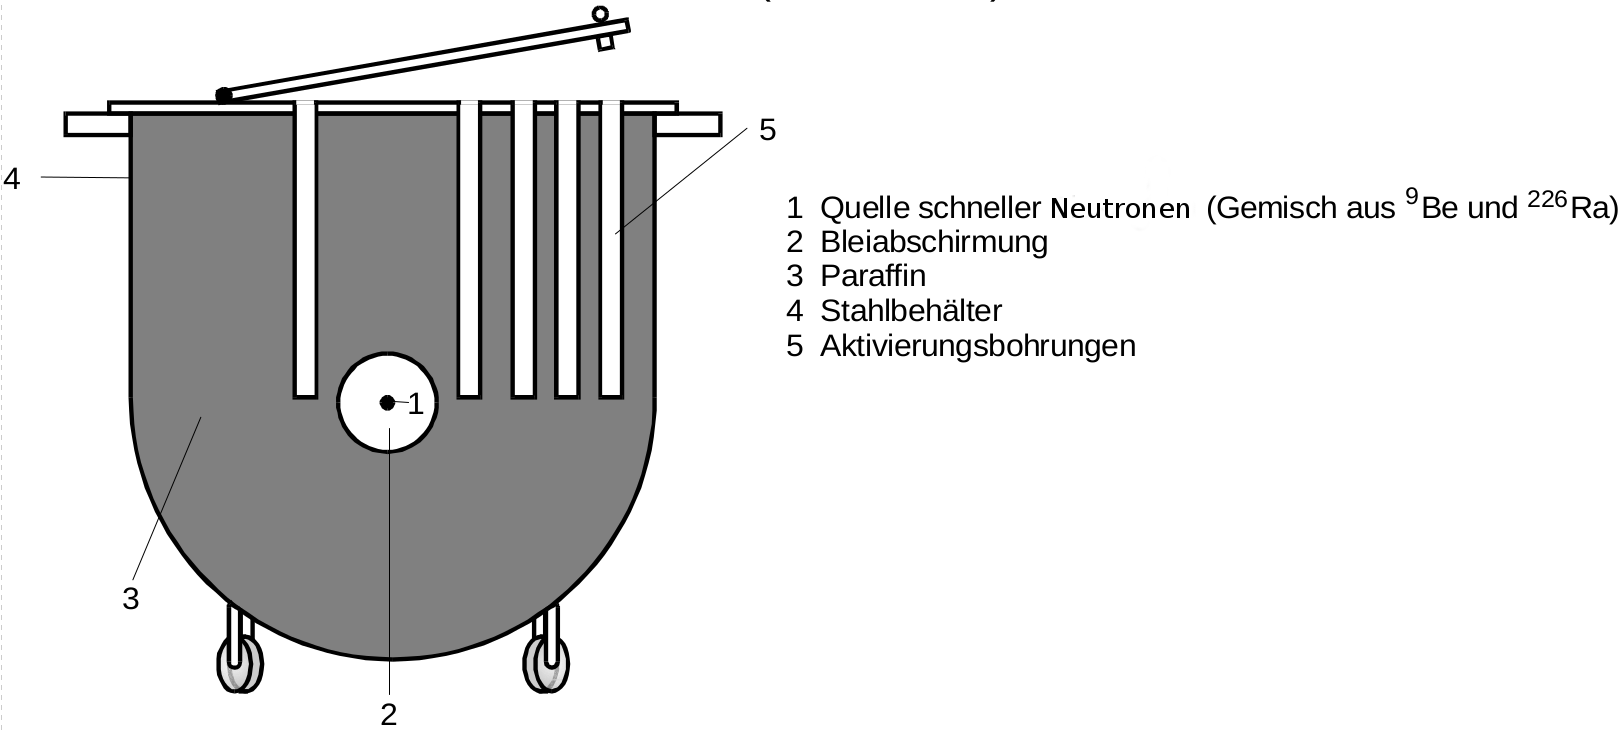
\includegraphics[width=\linewidth-70pt,height=\textheight-70pt,keepaspectratio]{content/kochtopf.png}
 \caption{Eine schematische Darstellung des Isotopenanreicherungbehälters \cite{V702}}
 \label{fig:topf}
\end{figure}


Der Messaufbau besteht im Kern aus einem radioaktiven Isotop und einem
 Geiger-Müller-Zählrohr, welches die auftretenden Zerfälle registriert. Dieses besteht aus einer mit Argon gefüllten Röhre. Trifft nun ein Betateilchen oder ein Gammaquant auf das Argon, wird dieses ionisiert und sorgt aufgrund einer hohen anliegenden Spannung für eine Elektronenlavine. Die Spannung kann anschließend ohne einen größeren Verstärker gemessen werden. Die Messzeit kann am Ausgabegerät des Zählrohrs eingestellt werden. Nach einem Durchlauf wird auf ein zweites Zählwerk gewechselt, sodass die aktuellen Ergebnisse notiert werden können. Zusätzlich ist der Messaufbau mit einer Bleikleidung versehen. Zum einen schirmt Sie das Messgerät vor verfälschender kosmischer Strahlung ab, zum anderen schützt Sie den Anwender vor der vorherrschenden Radioaktivität. Um die benötigten radioaktiven Isotope zu erzeugen, werden stabile Kerne in einem Behälter nach Abb. \ref{fig:topf} mit Neutronen beschossen. Um die Ausbeute zu maximieren durchlaufen die Neutronen zunächst jedoch eine bremsende Paraffinschicht.
